\todo{todo}
to mention:
google app engine
android stuff, api for graphs, others?
arduino code detail?


The software consist of two components. One cloudservice and one android client.

\begin{figure}
\centering
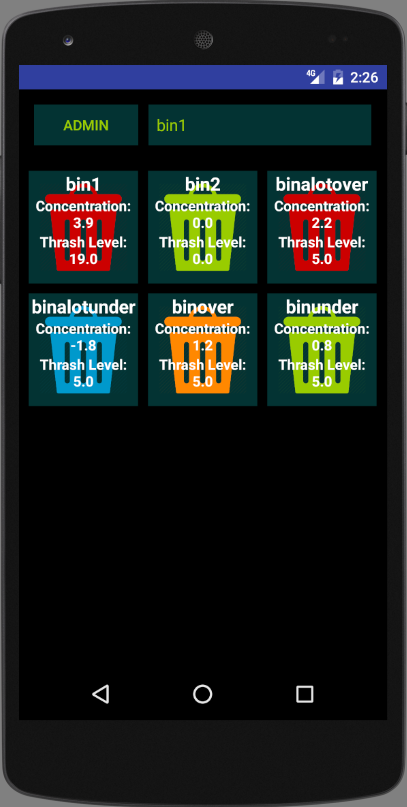
\includegraphics[scale=.3]{img/screen_admin}
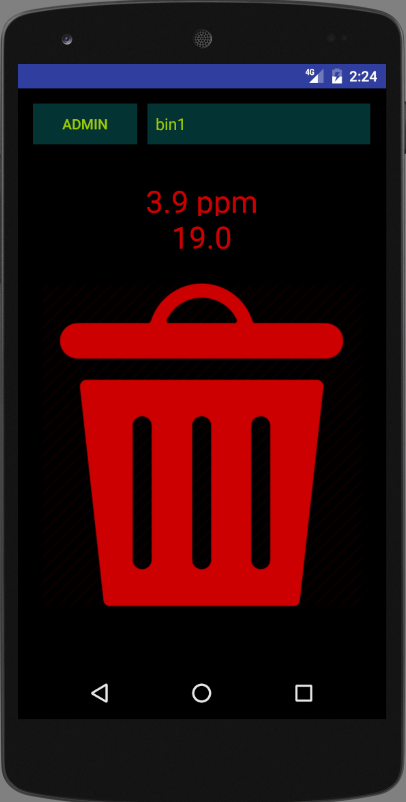
\includegraphics[scale=.3]{img/screen_single}
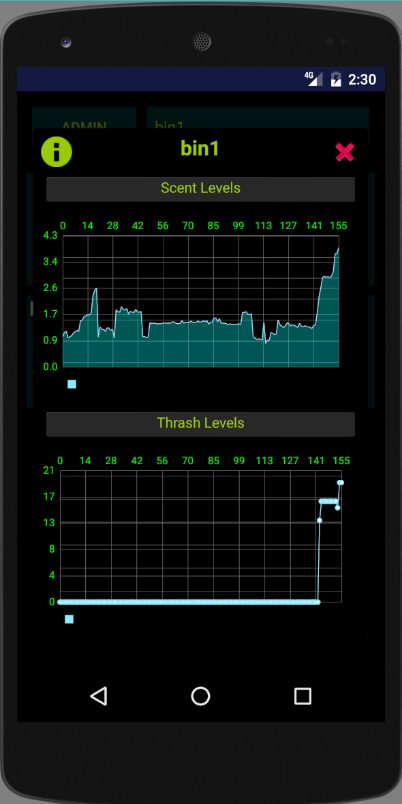
\includegraphics[scale=.3]{img/screen_stats}
\caption{Image of the three main views in the android client} 	
\label{fig:clientmodes}
\end{figure}

\begin{figure}
\centering
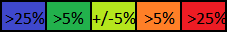
\includegraphics{img/app_colors_nb}
\caption{Image of the color codes ranging, from deviation under the norm to deviation over the norm} 
\label{fig:colorcodes}
\end{figure}


The android client can provide statistics about different smartbins - it only supports  presentation of data in its current form.
It supports two modes: \textbf{Admin mode} and \textbf{Single Bin mode}.
Admin mode includes overview of every single bin and graphs for each bin. The graphs are only available as long as enough context information is present see figure~\ref{fig:clientmodes}.

 Single bin mode provides a view of the current bin state.
 
 The bin state is divided into five different categories, this is represented visually as colors.
 The order is, \textit{blue}, \textit{dark green}, \textit{green}, \textit{orange}, and \textit{red}, as seen on figure~\ref{fig:colorcodes}.
The middle one, \textit{green}, is when the concentration is deviating with at most 5\%, next tier \textit{dark green} and \textit{orange} is a deviation of at most 25\%, and the last ones \textit{blue} and \textit{red} are deviations above 25\%.